% presentaion of On the Statistics of Macrospicules
\documentclass{beamer}
\mode<presentation>
\usepackage{graphicx}
\usepackage{float}
\usepackage{lmodern}
\usepackage{subcaption}

% The basic information needed to create a title page
\title{Macrospicules, Jets and the Solar Chromosphere}
\author{Samuel Bennett}
\institute{Solar Physics and Space Plasma Research Centre (SP$^2$RC) \\ University of Sheffield}
\date{21|${^st}$ November 2016}

\usetheme{Berlin} % Standard Blue in your face theme
\renewcommand{\bibname}{References}


% paper references
\newcommand*\aap{A\&A}
\let\astap=\aap
\newcommand*\aapr{A\&A~Rev.}
\newcommand*\aaps{A\&AS}
\newcommand*\actaa{Acta Astron.}
\newcommand*\aj{AJ}
\newcommand*\ao{Appl.~Opt.}
\let\applopt\ao
\newcommand*\apj{ApJ}
\newcommand*\apjl{ApJ}
\let\apjlett\apjl
\newcommand*\apjs{ApJS}
\let\apjsupp\apjs
\newcommand*\aplett{Astrophys.~Lett.}
\newcommand*\apspr{Astrophys.~Space~Phys.~Res.}
\newcommand*\memsai{Mem.~Soc.~Astron.~Italiana}
\newcommand*\solphys{Sol.~Phys.}
\newcommand*\ssr{Space~Sci.~Rev.}
\newcommand*\nat{Nat.~Lett.}
\newcommand*\pasj{def}



\begin{document}

	\begin{frame}
	\maketitle
		\begin{minipage}{0.3\textwidth}
			\begin{flushleft}
				
\includegraphics[width=0.8\textwidth]{Figs/University_Crest.pdf}
			\end{flushleft}
		\end{minipage}
		\begin{minipage}{0.3\textwidth}
			\begin{center}
				
\includegraphics[width=0.5\textwidth]{Figs/SP2RC.pdf}
			\end{center}
		\end{minipage}
		\begin{minipage}{0.3\textwidth}
			\begin{flushright}
			%\includegraphics[width=0.8\textwidth]{Figs/SWAT.pdf}
			\end{flushright}
		\end{minipage}
	\end{frame}


%Background of Macrospicules
	\begin{frame}{Spicules}
		\begin{itemize}
			\item{Story begins with Spicules}
			\item{Discovered by Angelo Secchi in 1887}
		\end{itemize}
%		\begin{figure}
%			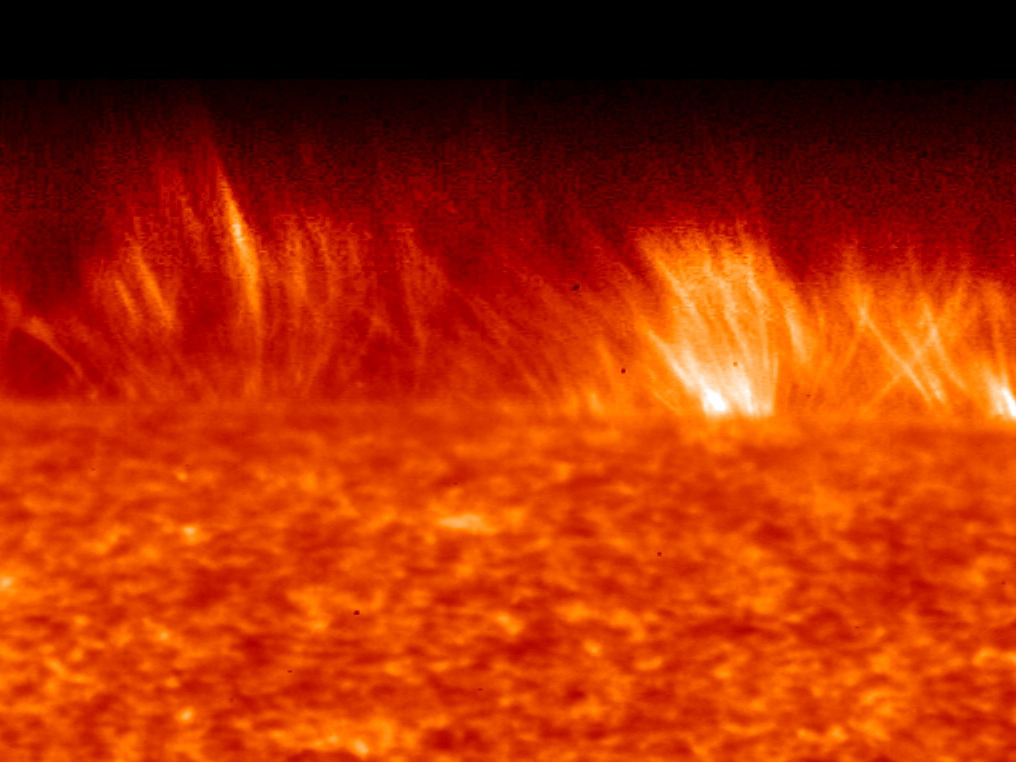
\includegraphics[scale=0.3]{Figs/spicules_at_limb.jpg}
%			\caption{SDO $30.4$ nm, NASA}
%		\end{figure}
	\end{frame}


%More background
	\begin{frame}{Early Work}
		\begin{itemize}
			\item{First observations by \cite{Bohlin1975}}
				\begin{itemize}
				\item{Lifetimes of $5 - 40$ min and lengths of $5 - 60$ arcsec}
				\end{itemize}
			\item{Similarly observed by \cite{Godoli1967} in H$\alpha$ but were described as bright surges on the limb, work which was followed up by \cite{LaBonte79}}	
			\item{There is some debate as to whether EUV and H$\alpha$ macrospicules are part of the same feature or are in fact two separate features.} 
		\end{itemize}	
	\end{frame}

% Further papers, not sure how nessesary this slide would be but hey
	\begin{frame}{Advancement}
		\begin{itemize}
			\item{\cite{Dere89} presents these features using the Spacelab 2 mission}
				\begin{itemize}
					\item{Don't find the extreme examples from \cite{Bohlin1975}}
					\item{Length $5 - 23$ arcsec and lifetime of $\geq 3$ min}
				\end{itemize}
			\item{Studies in possible rotating motions were undertaken by \cite{Pike_Mason1998}}
			\item{There is also evidence for possible solar wind acceleration \cite{Pike_Harrison1997}}
				\begin{itemize}
					\item{Used the concept of multi-thermal structure i.e. a cool core with a hot sheath.}
					\item{These papers both used the CDS on-board SoHO} 
				\end{itemize}
			\item{\cite{Parenti2002} continued the examination of multi-thermal structure and the evolution of the macrospicule}
			\item{Spectroscopic investigation of macrospicules has begun, best example of which is \cite{Scullion2010}}
		\end{itemize}
	\end{frame}
	
	\begin{frame}{Formation Mechanisms}
		Differently to spicules, where the prevailing hypothesis presents p-mode leakage into the atmosphere, macrospicules are likely formed through larger scale mechanisms.
		\begin{itemize}
			\item{\cite{Shibata1992} demonstrate the standard model of X-ray jet mechanism.}
			\begin{itemize}
				\item{In this case, the primary cause of onset is flux emergence.}
				\item{Small scale loops rise through the solar convection zone and into the magnetically complex chromosphere.}
				\item{The result of this is that regions of opposite magnetic field come into contact, causing a violent release of magnetic tension.}
			\end{itemize}
			\begin{figure}
				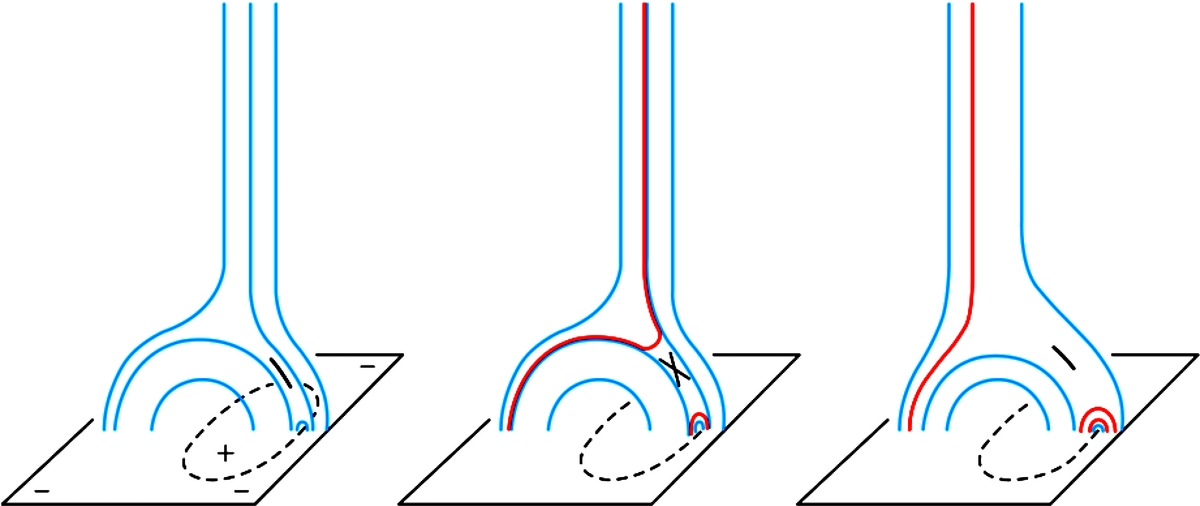
\includegraphics[scale=0.2]{Figs/inverted_Y.png}
				\caption{\cite{Moore2010}}
			\end{figure}
		\end{itemize}
	\end{frame}

	\begin{frame}{Formation Mechanisms}
		\begin{itemize}
			\item{In the inverted Y scenario, the emerging flux is in a twisted state.}
			\item{\cite{Moore2010} present a dichotomy of coronal jets.}
			\item{In this case there is a lack of twist in the underlying magnetic field.}
			\item{The result of which, is the 'curtain' of plasma emerging from the reconnection site.}
			\begin{figure}
				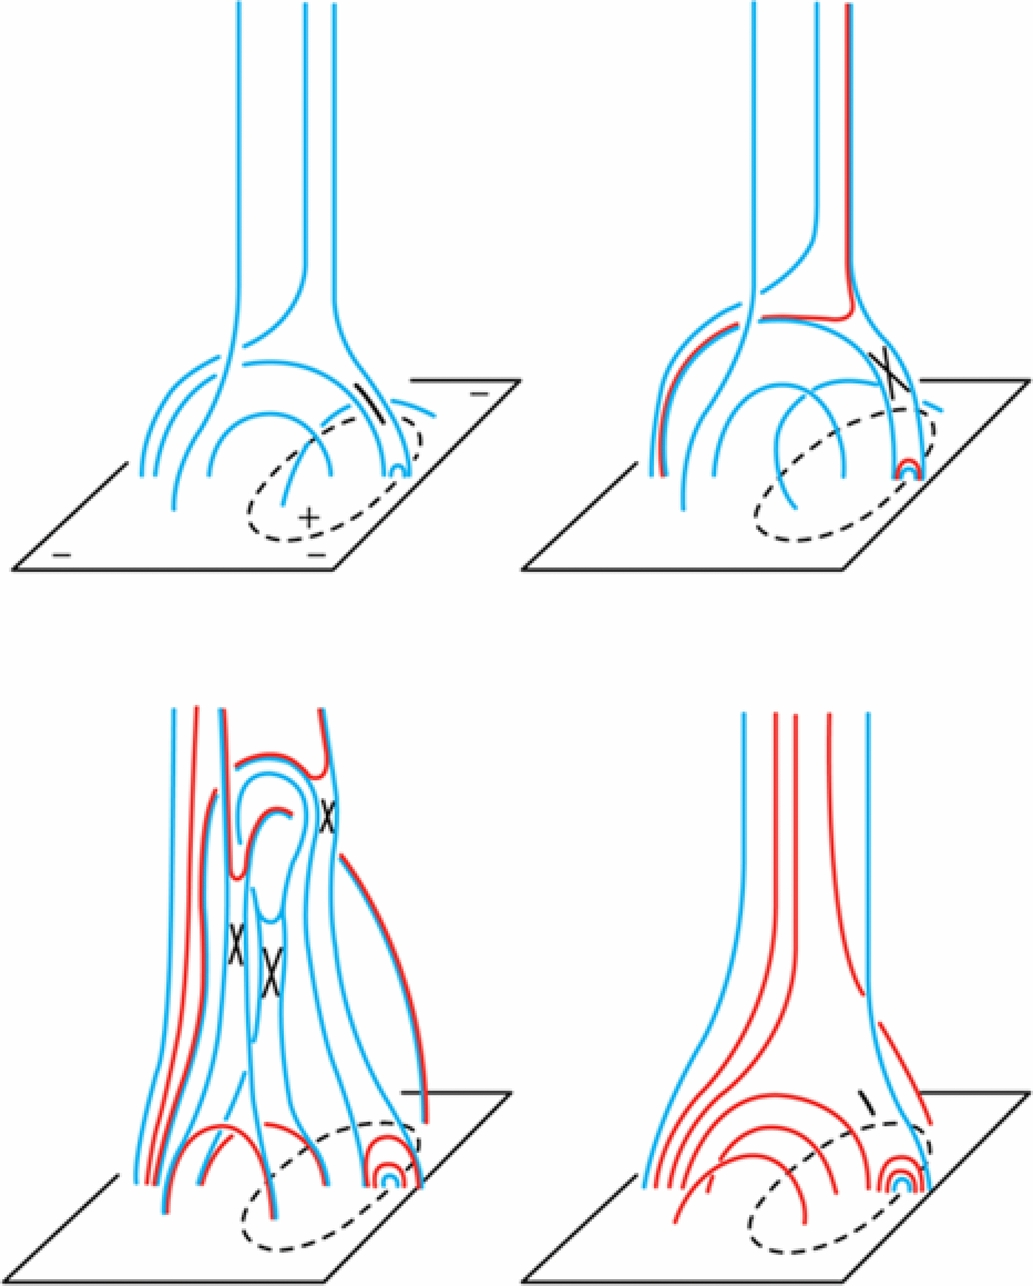
\includegraphics[scale=0.2]{Figs/blowout_jet.png}
				\caption{\cite{Moore2010}}
			\end{figure}
		\end{itemize}
	\end{frame}
	
	
% Motivation for the work
	\begin{frame}{Motivation for studying macrospiules}
		\begin{itemize}
			\item{Clarifying the macrospicules place in the solar ejecta}
			\item{Any possible implications for coronal heating}
			\item{A feature which originates in the photosphere/chromosphere but extends into the corona}
		\end{itemize}
	\end{frame}		


	\begin{frame}{A Breif Outline}
		\begin{itemize}
			\item An example of a macrospicule from the sample
		\end{itemize}
	\begin{figure}
		\begin{center}
			\begin{subfigure}[b]{0.3\textwidth}
				\begin{center}
					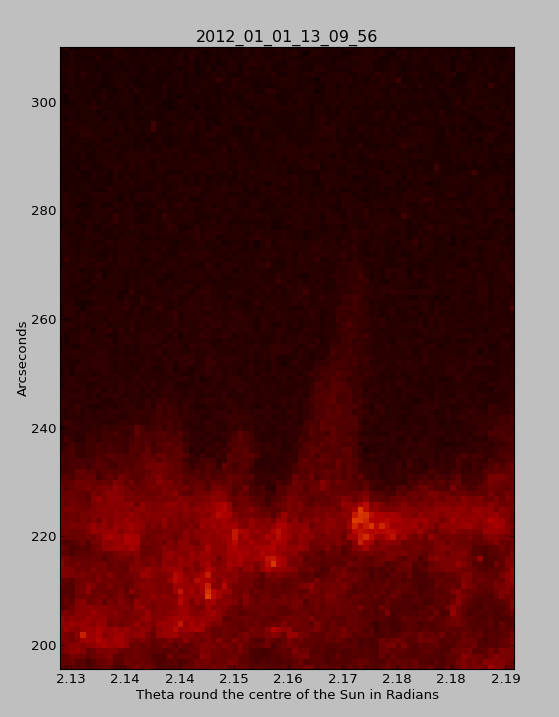
\includegraphics[width=\textwidth]{Figs/example_ms.png}
				\end{center}
			\end{subfigure}
			\begin{subfigure}[b]{0.495\textwidth}			
				\begin{center}
					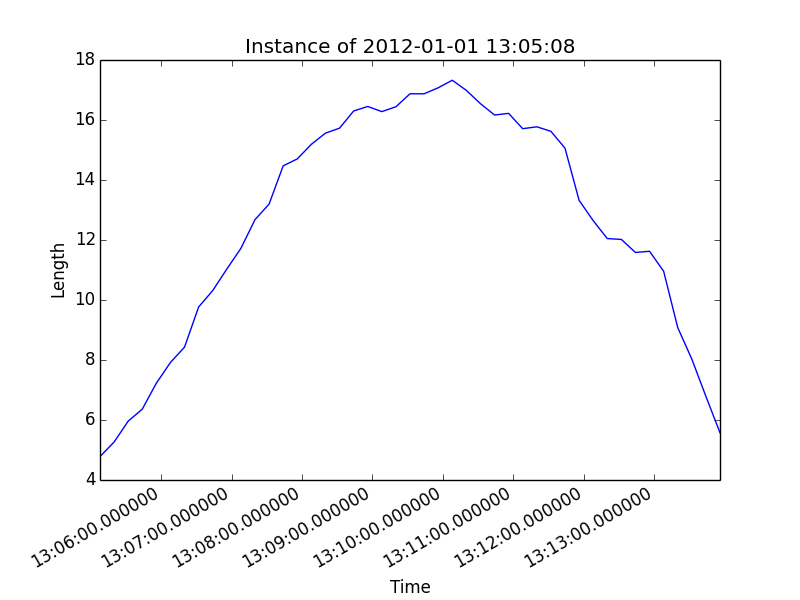
\includegraphics[width=\textwidth]{Figs/example_evo.png}
				\end{center}
			\end{subfigure}			
		\end{center}
	\end{figure}
	\end{frame}

	
	\begin{frame}{The Work}
		\begin{itemize}
			\item The aim of the work is to define a set of characteristic properties for macrospicules
				\begin{itemize}
					\item Spatial, temporal and statistical
				\end{itemize}
			\item Using the AIA $30.4$ nm on-board SDO.
			\item Cadence of $12$ s and resolution of $0.6$ arcsec per pixel 
			\item Utilizing the full length of SDO's operations, giving a $2$ $1/2$ year sample period
				\begin{itemize}
					\item Taking a two hour sample on the $1$st and $15$th of every month 
				\end{itemize}
			\item The limb of the Sun was flattened out and the length and width of the features were measured
			\item Survey used samples which had full parabolic evolution's and lengths up to $200$ arcsec in length
		\end{itemize}
	\end{frame}


	\begin{frame}{Basic Properties}
	% Basic property histograms
		\begin{figure}
				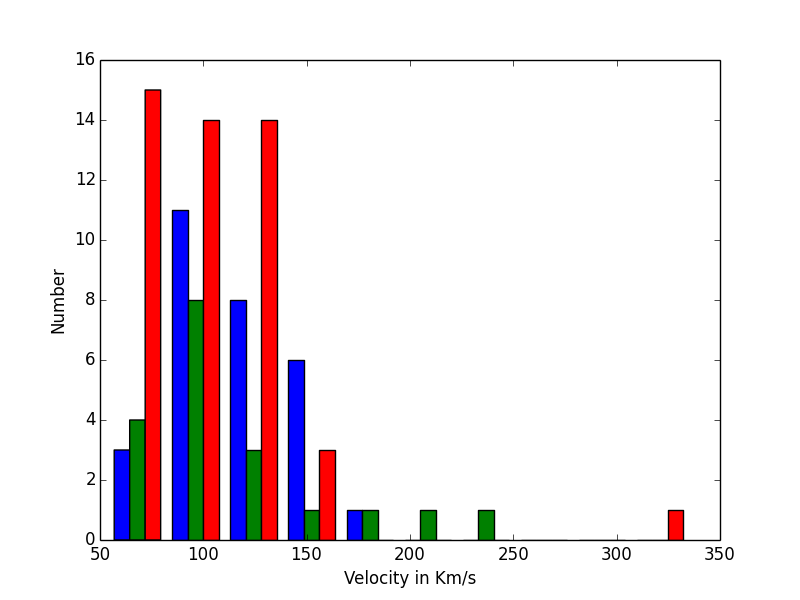
\includegraphics[scale=0.20]{Figs/vel_hist.png}
				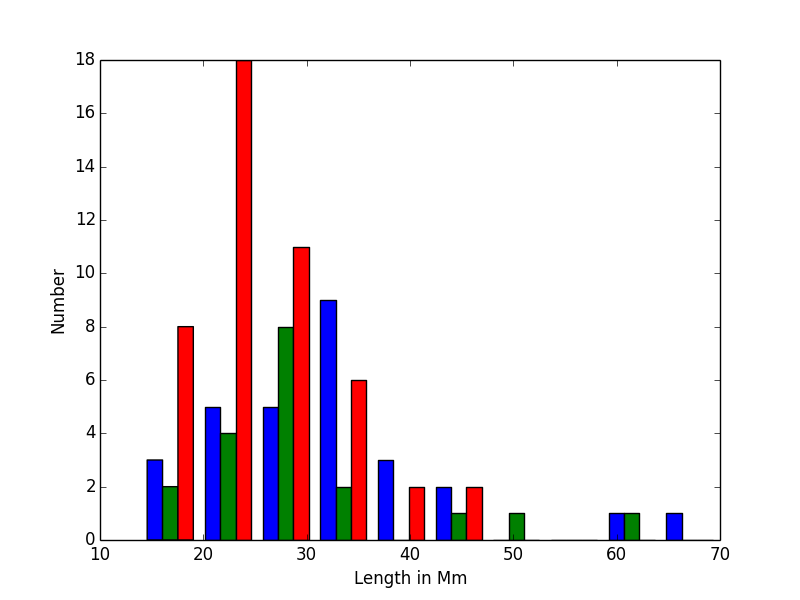
\includegraphics[scale=0.20]{Figs/len_hist.png}\\
				
				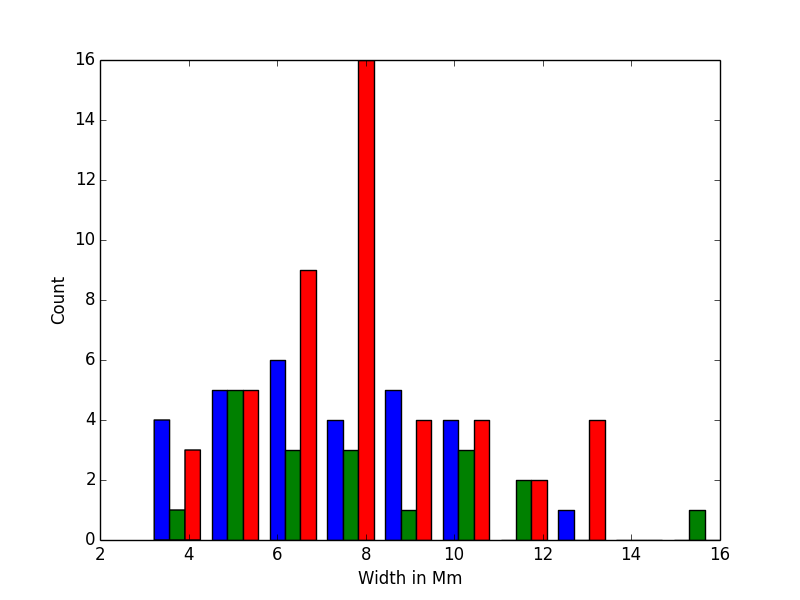
\includegraphics[scale=0.20]{Figs/width_hist.png}
				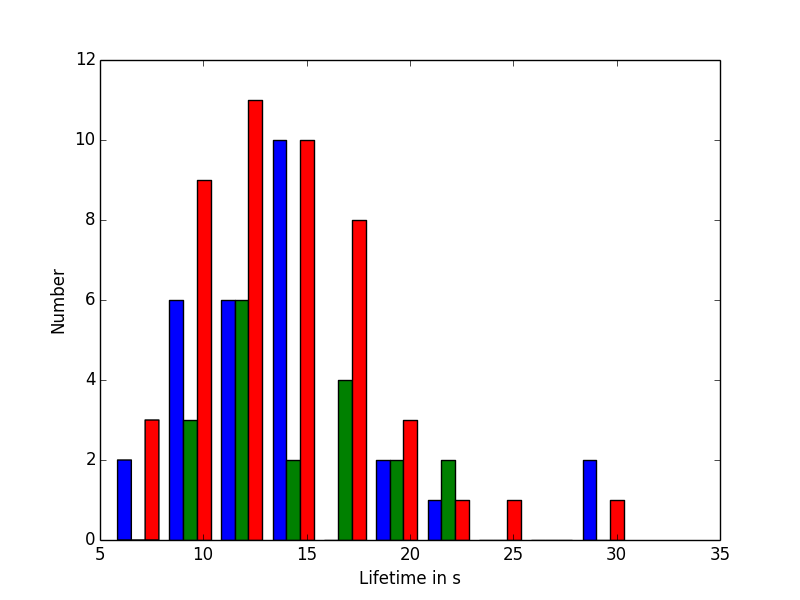
\includegraphics[scale=0.20]{Figs/lt_hist.png}
		\end{figure}
	\end{frame}
	
	\begin{frame}{Inclination and Latitude}
	% Inclination vs latitude
		\begin{itemize}
			\item{Coronal Hole (CH), Coronal Hole Boundaries (CHB) and Quiet Sun instances}
			\item{Notable is the clear difference between inclination of CH and CHB macrospicules}
		\end{itemize}
		\begin{figure}
			\centering
				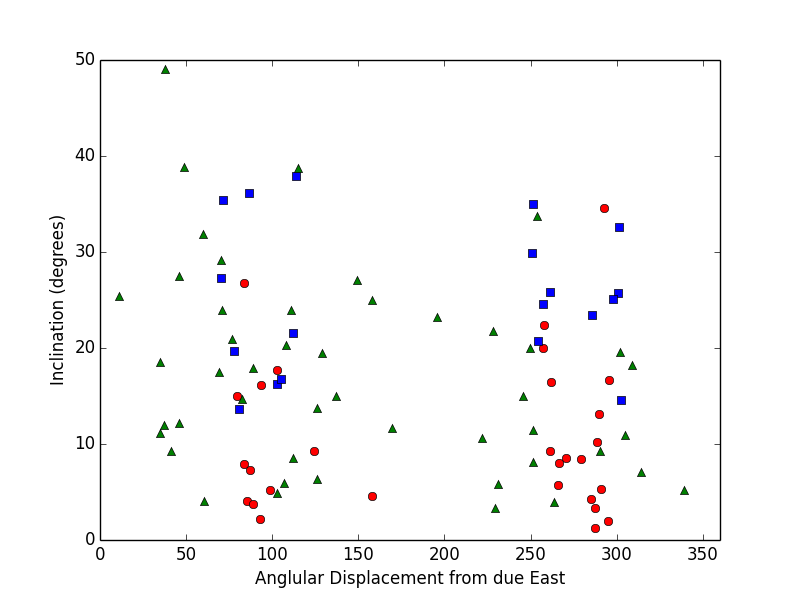
\includegraphics[scale=0.25]{Figs/tilt_vs_lat.png}
		\end{figure}
	\end{frame}
	
	
	
	\begin{frame}
		\begin{center}
			Is there a correlation between the basic properties?			
		\end{center}

	\end{frame}
	
	
	
	\begin{frame}
		\begin{minipage}{0.49\textwidth}
			\begin{flushleft}
				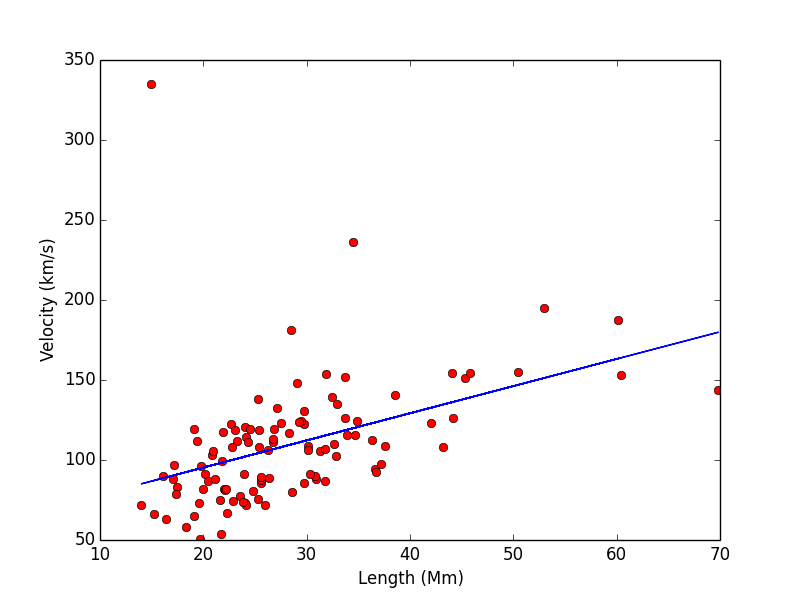
\includegraphics[width=1\textwidth]{Figs/length_max_vs.png}
			\end{flushleft}
		\end{minipage}
		\begin{minipage}{0.49\textwidth}
			\begin{center}
				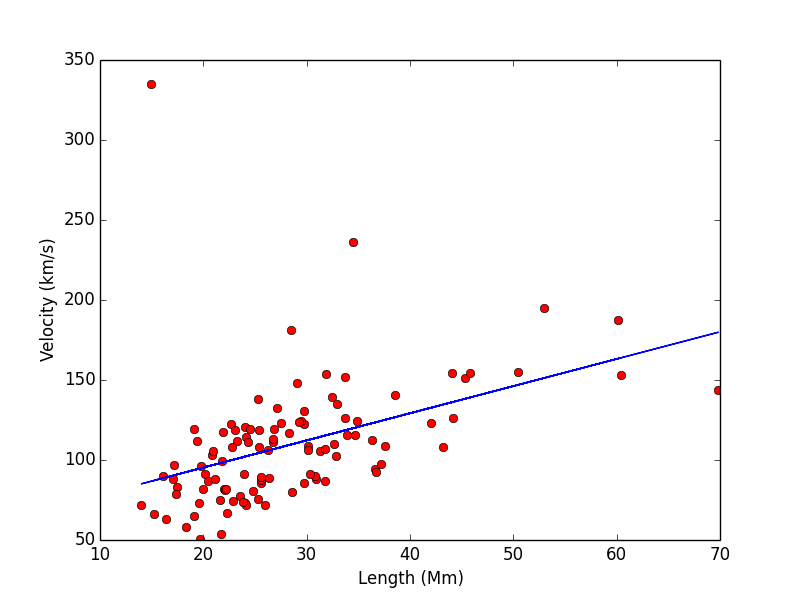
\includegraphics[width=1\textwidth]{Figs/length_max_vs.png}
			\end{center}
		\end{minipage}\\
		\begin{minipage}{0.49\textwidth}
			\begin{flushright}
			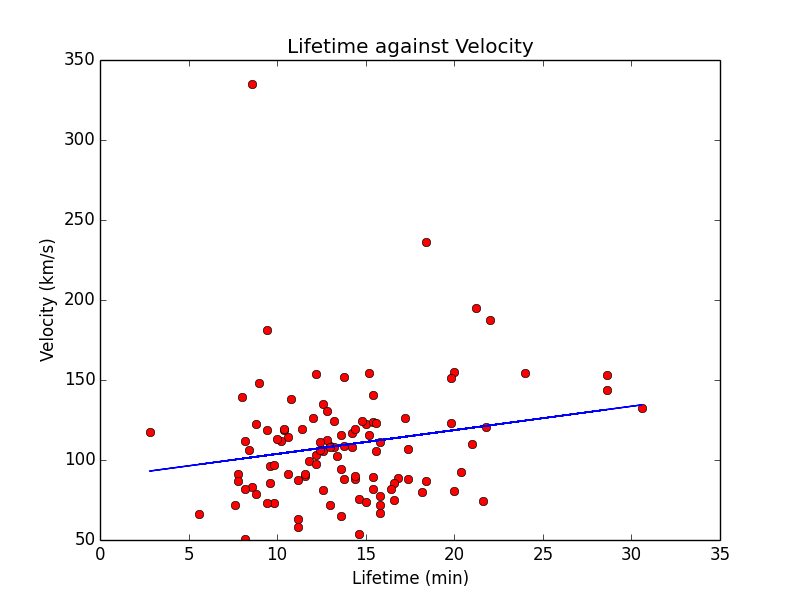
\includegraphics[width=1\textwidth]{Figs/velocity_vs_lt.png}
			\end{flushright}
		\end{minipage}
		\begin{minipage}{0.49\textwidth}
			\begin{itemize}
				\small
				\item{Top left, v=61.3(1+0.28L)}
				\item{Top right, L=10.39(1+0.12T)}
				\item{Bottom left, v=88.9(1+0.016)}
			\end{itemize}
		\end{minipage}
	\end{frame}


	
	\begin{frame}
		\begin{minipage}{0.49\textwidth}
			\begin{flushleft}
				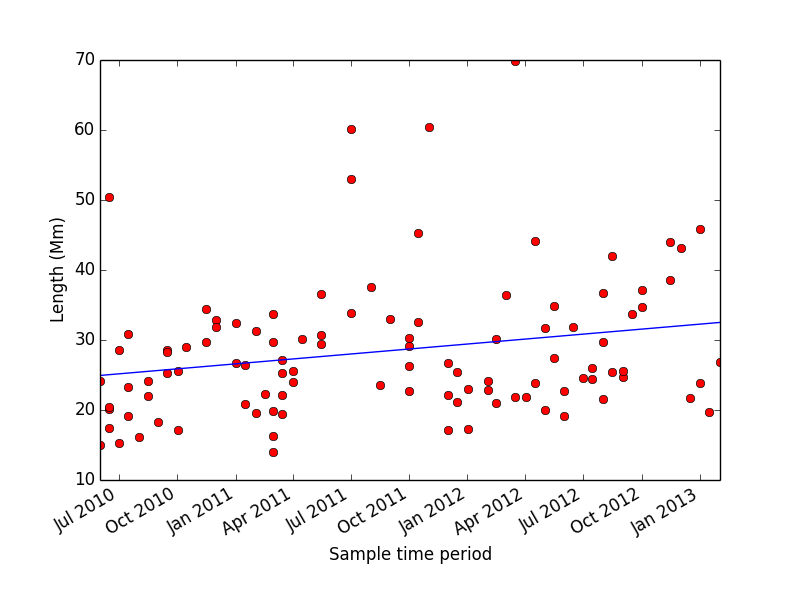
\includegraphics[width=1\textwidth]{Figs/length_vs_solarcycle.png}
			\end{flushleft}
		\end{minipage}
		\begin{minipage}{0.49\textwidth}
			\begin{center}
				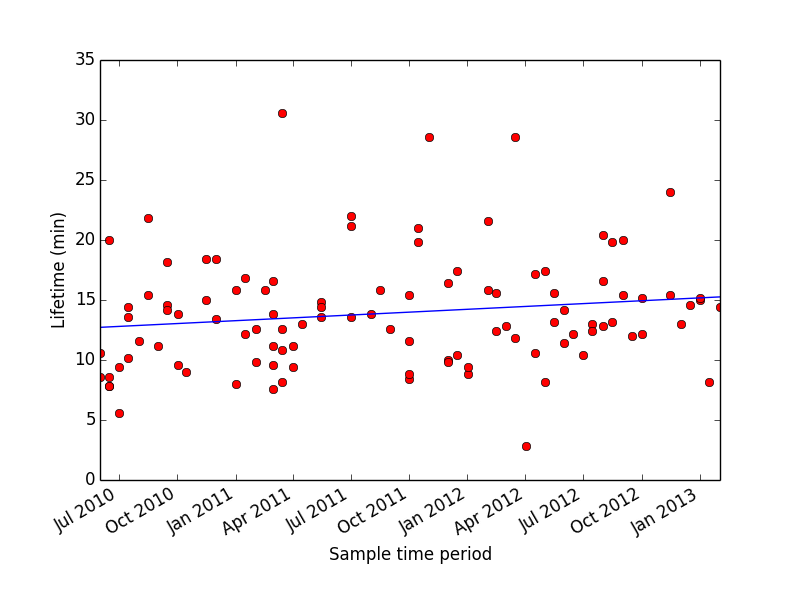
\includegraphics[width=1\textwidth]{Figs/life_vs_solarcycle.png}
			\end{center}
		\end{minipage}\\
		\begin{minipage}{0.49\textwidth}
			\begin{flushright}
			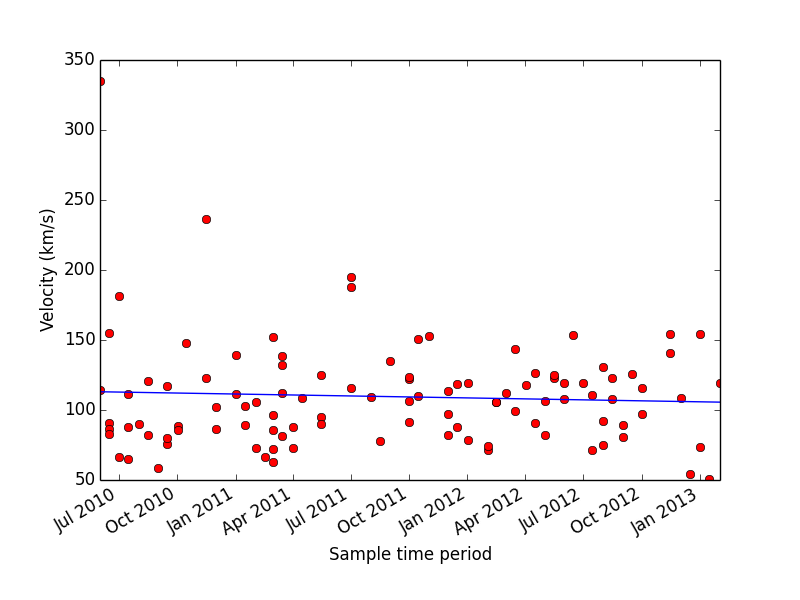
\includegraphics[width=1\textwidth]{Figs/velocity_vs_solarcycle.png}
			\end{flushright}
		\end{minipage}
		\begin{minipage}{0.49\textwidth}
			\begin{itemize}
				\small
				\item{top left L=24.9(1+0.11t)}
				\item{top right T=12.7(1 + 0.074t)}
				\item{lower left V=113.03(1-0.025t)}
			\end{itemize}
		\end{minipage}
	\end{frame}






	\begin{frame}{Ballistics and energetics}
		\begin{itemize}
			\item{Width decreases after the apex of the macrospicules trajectory}
			\item{Time taken for the macrospicules to fall, significantly greater than would be expected.}
		\end{itemize}
		
		\begin{figure}
			\centering
				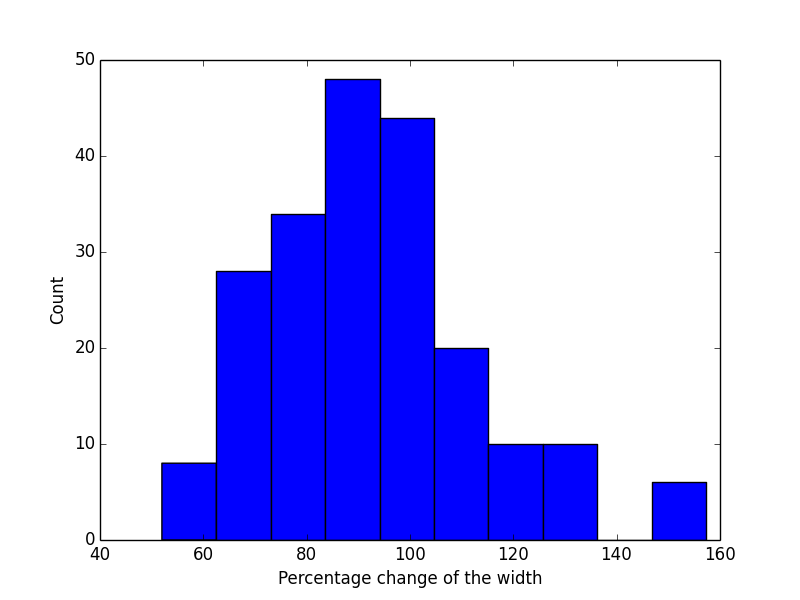
\includegraphics[scale = 0.25]{Figs/width_percent.png}
				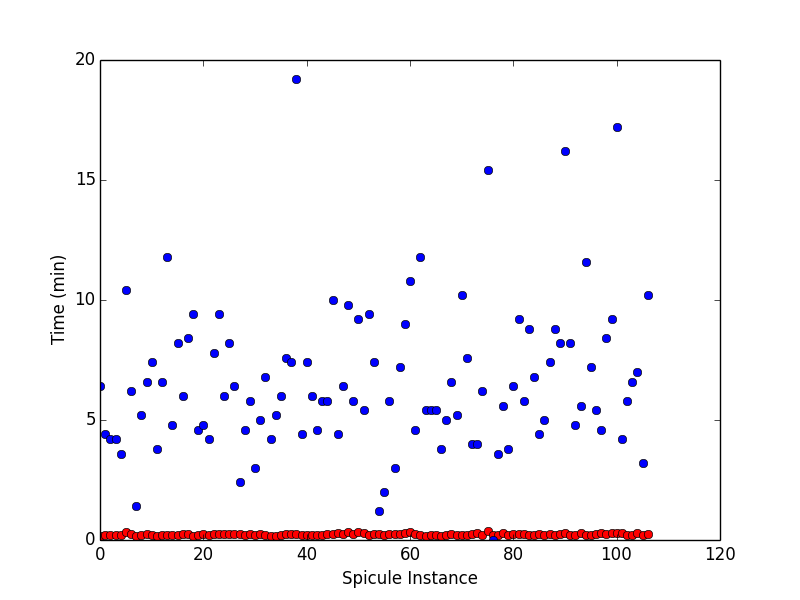
\includegraphics[scale = 0.25]{Figs/times_falling.png}
		\end{figure}
	\end{frame}
	
	\begin{frame}{Ballistics and energetics}
		Possible energy transfer into the corona?
		\begin{itemize}
			\item{The amount of energy that could possibly be transferred into the corona, would be related to the amount of energy required to generate the macrospicule in the first place}
			\item{Therefore the mass of the macrospicule must be estimated}
			\item{Using the density of the photosphere and the corona as $\rho_0$ and $\rho$, the centre of mass was estimated}
			\item{The amount of mechanical energy within the macrospicule was then estimated as the amount of energy required to move this mass from the limb to the centre of mass}
		\end{itemize}
	\end{frame}	
	
	\begin{frame}{Ballistics and energetics}
		\begin{itemize}
			\item{Estimates of the energy for each scale height}
		\end{itemize}
		\begin{figure}
			\centering	
				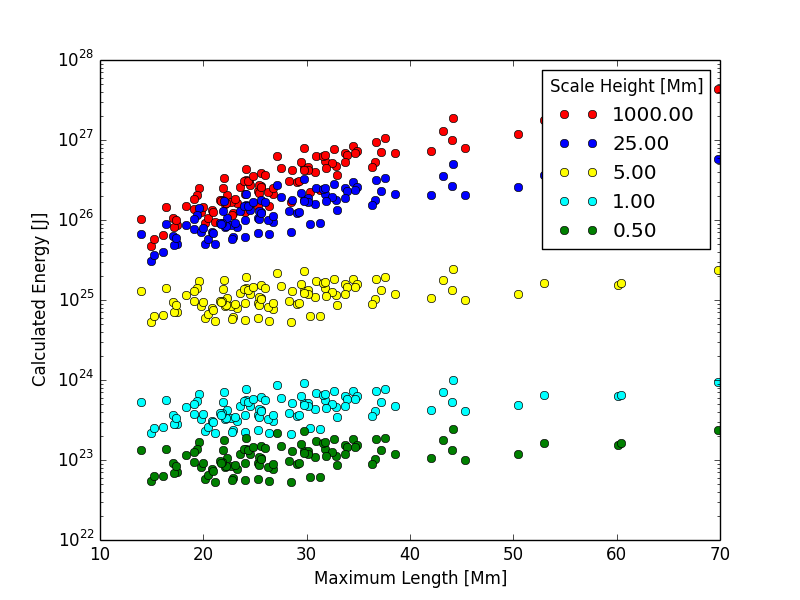
\includegraphics[scale = 0.35]{Figs/scale_h.png}
		\end{figure}
	\end{frame}


	\begin{frame}{Round-up}
			\begin{itemize}
				\item Spatial properties
				\begin{itemize}
					\item \textbf{Length} with range $14.0$ - $69.0$ Mm with a mean of $48.4$ Mm
					\item \textbf{Width} has a range of $3.1$ - $16.1$ Mm and mean of $7.6$ Mm
					\item \textbf{Maximum Velocity} range is $54.1$ - $335.5$ km/s and a mean of $109.7$ km/s 
				\end{itemize}
				\item \textbf{Lifetimes} in this case are in a range $2.7$ - $30.6$ min and mean of $13.9$ min
				\item{Widths become smaller after the peak of their trajectory}
				\item{Fall back to limb time is slower than expected}
				\item{If even 1\% of the energy used to form a macrospicule is transferred into the corona they are an exellent candidate for a heating source}
	
			\end{itemize}
	\end{frame}
	
	
	
%%%%%%%%%%%%%%%%%%%% case study section

	\begin{frame}{A Case Study}
		\begin{itemize}
			\item{We aim to build a comprehensive description of a macrospicule}
			\item{The macrospicule in question occurs on $21/06/2012$.}			
			\begin{itemize}
				\item{The feature was observed by the Swedish Solar Telescope (SST) using the CRISP instrument.}
				\item{This gives us a $32$ spectral increments from $H\alpha$.}
				\item{We also observe the feature in SDO/AIA and STEREO/EUVI allowing us to build a much larger picture.}
			\end{itemize}
			\item{Alas, Hinodes XRT is in power-down mode as the feature forms, depriving us of this potentially crucial information.}
		\end{itemize}
	\end{frame}	
	
	\begin{frame}
		\begin{itemize}
			\item{Using the tool we built for the first study, we have analysed the AIA images.}
			\item{The feature is visible in all the lines above the chromosphere.}
			\begin{itemize}
				\item{$30.4$, $33.5$, $21.1$, $17.1$ and $13.1$ nm.}
				\item{It was also applied to the $H\alpha$ images.}
				\item{The result is that we observe the evolution of the feature throughout the atmosphere.}
			\end{itemize}
		\end{itemize}
			\begin{figure}
				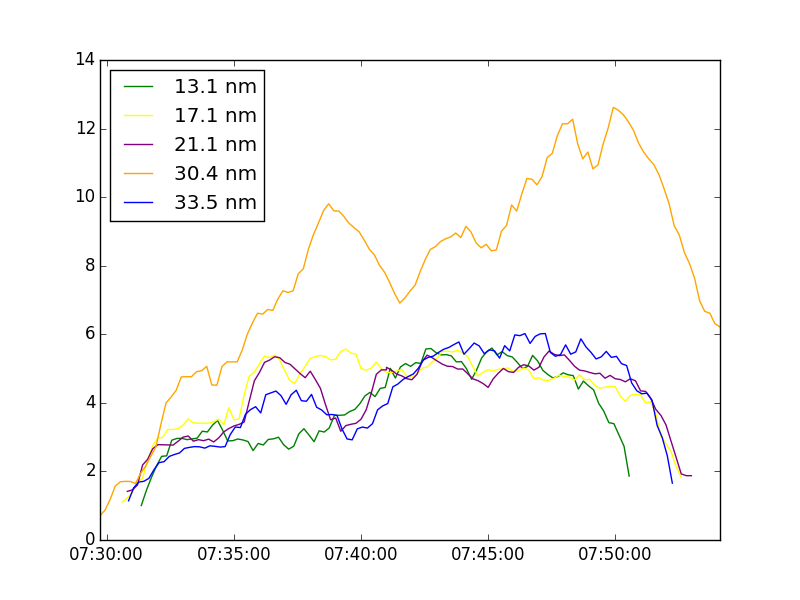
\includegraphics[scale=0.32]{Figs/len_plot.png}
			\end{figure}

	\end{frame}
	
	\begin{frame}
		\begin{itemize}
			\item{Notice that the extent of the feature is greatest in the lower wavelengths, H$\alpha$ and $30.4$.}
		\end{itemize}
			\begin{itemize}
				\item{There are two clear peaks in the length with a recession between}
				\item{Leading to the possible conclusion that there are two separate acceleration events}
			\end{itemize}
	\end{frame}
	
% moar images here for brigding over the figures

	\begin{frame}
		% image frame
	\end{frame}


	\begin{frame}
		\begin{itemize}
			\item{Notice that the extent of the feature is greatest in the lower wavelengths, H$\alpha$ and $30.4$.}
			\begin{itemize}
				\item{There are two clear peaks in the length with a recession between.}
				\item{Leading to the possible conclusion that there are two separate acceleration events.}
			\end{itemize}
			\item{However, the feature does not reach as high in any of the hotter emission lines.}
			\item{And we don't necessarily see the same 'double acceleration in all these lines.}
			\item{We record a maximum length of $12.1$ Mm.}
		\end{itemize}
	\end{frame}

	
	\begin{frame}{STEREO Images}
		\begin{itemize}
			\item{While this feature formed, the STEREO mission was at $90^\circ$ to the Sun-Earth line.}
			\item{As such we can investigate the appearance of our feature from a non Earth based perspective.}
			\item{Using a bit of trigonometry, we calculate the full extent of the feature.}
			\begin{itemize}
				\item{$\mathbf{25.5}$ Mm}
			\end{itemize}
		\end{itemize}
		% Stereo IMAGES
		\begin{figure}
			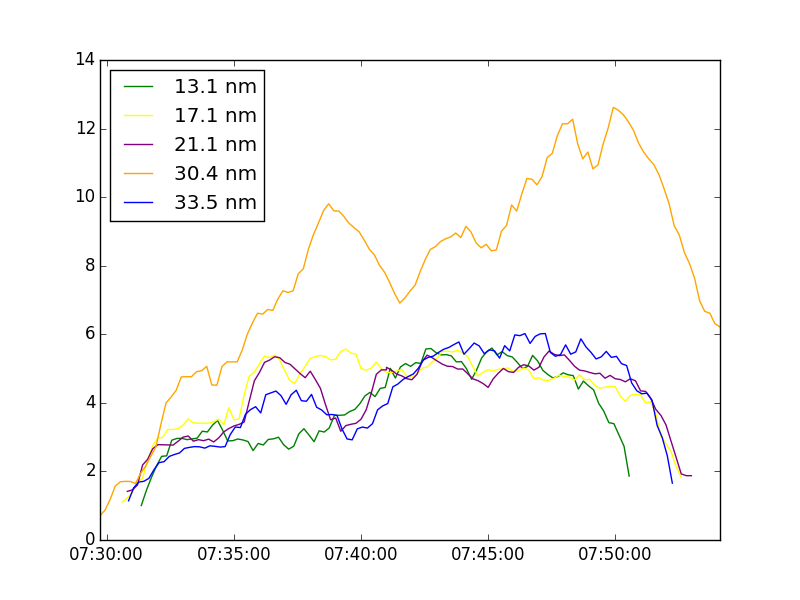
\includegraphics[scale=0.4]{Figs/len_plot.png}
		\end{figure}
	\end{frame}
	
	\begin{frame}{Dopplergram Analysis}
		\begin{itemize}
			\item{Given the fine spectroscopic data we have, H$\alpha$ core and $+0.2 -0.12$ nm, we can calculate the dopplershifts produced.}
			\item{We can do this by fitting the line profile over the full range.}
		\end{itemize}
	\end{frame}
	
%	\begin{frame}
%		\big{BUT}
%	\end{frame}

	\begin{frame}{Doppler-problems}
		\begin{itemize}
			\item{The line profiles in this region change, on-disk to off disk.}
			\begin{itemize}
				\item{On disk, the spectral line profile form is absorption.}
				\item{At the limb, the profile of the spectrum is emission.}
			\end{itemize}
			\item{As such, fitting the profile is difficult.}
			\item{Therefore}
		\end{itemize}
	\end{frame}
	
%	\begin{frame}
%		\big{Markov-Chain Monte-Carlo}
%	\end{frame}
	
	
	\begin{frame}{Markov-Chain Monte-Carlo Modelling}
		\begin{itemize}
			\item{We fit both single and double Gaussian line profiles.}
			\item{The primary issue is resolving between the two emission profiles.}
			\item{Therefore we fit a distribution of possible fits to both.}
			\item{Subsequently utilising a Bayesian Information Criterion allows differentiation between the two.}
		\end{itemize}
	\end{frame}

	\begin{frame}{Doppler Velocities}
		\begin{itemize}
			\item{Then, by minimising the two distributions and applying the Doppler equation, we can calculate the LoS velocity of the feature.}
			\item{During the first acceleration of the feature, no prominent LoS motion was detected.}
			\item{However during the second acceleration of plasma, we notice some very distinctive behaviour.}
		\end{itemize}
	\end{frame}

	\begin{frame}
		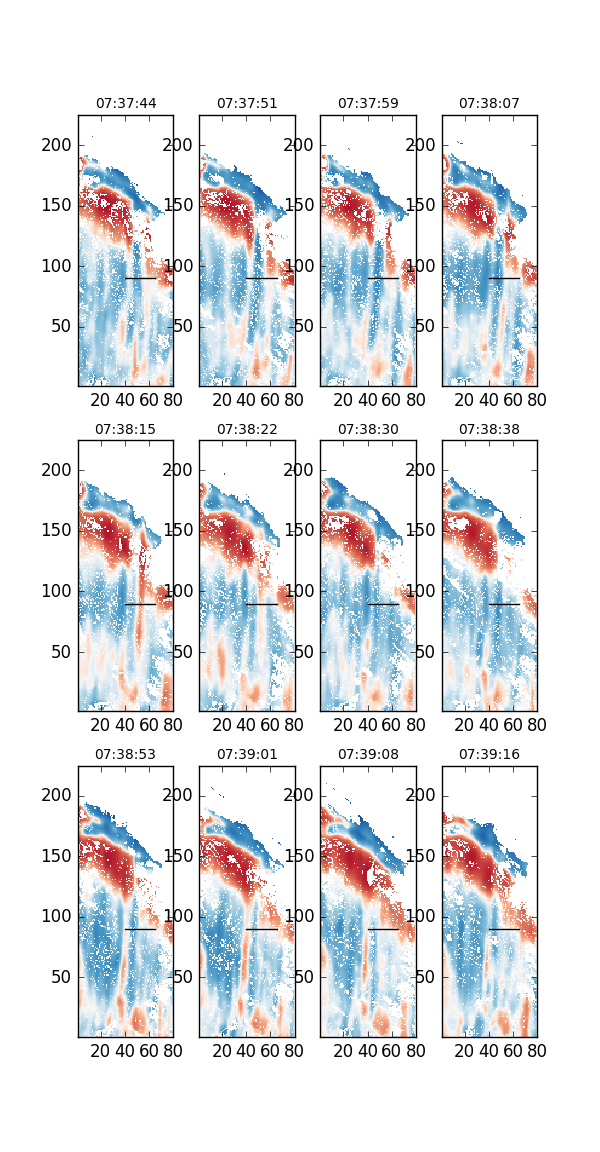
\includegraphics[scale=0.5]{Figs/dopplergram.png}
	\end{frame}

	\begin{frame}{Doppler Velocities}
		\begin{itemize}
			\item{The feature extends upwards during the acceleration phase, looses momentum, and begins to 'unwind' from the tip of the feature.}
			\item{The redshift then takes over the motion of the entire feature.}
			\item{After a while the magnetude of this velocity decreases and the feature appears to leave the images.}
			\item{However, in its place, appears blue shift and the feature proceeds to rotate in the opposite direction.}
		\end{itemize}
	\end{frame}

	\begin{frame}{Conclusions}
		\begin{itemize}
			\item{The feature is clearly visible in $H\alpha$ and $30.4$ nm and follows the behaviours of a macrospicule as found in the statistical analysis.}
			\item{This lends credence to the argument that the two are the same feature. Forming out of the same physical mechanism.}
			\item{This macrospicule appears to be formed from the standard jet mechanism highlighted by Shibata et al.1992}
			\item{It displays torsional motion consistent with an inherent magnetic field, suggesting reconnection even more as a formation mechanism.}
		\end{itemize}
	\end{frame}


% % % % % % % % concluding 

	\begin{frame}{Conclusion}
	content...
	\end{frame}

	\begin{frame}{References}
	\tiny
	\bibliographystyle{authordate1}
	\bibliography{references}
	\end{frame}


\end{document}